% =============================================================================
% Capítulo 4 — Metodologia: Pré-processamento e Engenharia de Características
% =============================================================================


Este capítulo descreve a metodologia adotada para desenvolver o \textbf{fluxo de trabalho em etapas} (\textit{pipeline}) de detecção automatizada de ocultações estelares em curvas de luz. A exposição está organizada em etapas sucessivas: desde a aquisição e o armazenamento dos dados até o \textbf{treinamento} (ajuste dos parâmetros dos classificadores) e a \textbf{avaliação} (medida do desempenho em dados não usados no ajuste). 

Os objetivos deste capítulo são: (1) descrever a arquitetura completa da \textit{pipeline}, da coleta dos dados ao modelo treinado; (2) detalhar o pré-processamento das curvas de luz, incluindo fontes de dados, armazenamento em banco relacional, normalização e critérios de classificação; (3) explicar a construção do conjunto de dados utilizado no treinamento, incluindo o recorte de segmentos negativos a partir de curvas positivas e a incorporação de curvas sintéticas; (4) formalizar a engenharia de características (\textit{feature engineering}) aplicada às curvas; e (5) especificar o protocolo de treinamento e avaliação dos classificadores, com as métricas e a divisão treino/teste adotadas. Ao final, o leitor terá uma visão clara de como os dados brutos são transformados em um conjunto de atributos e como os modelos são treinados e avaliados, preparando o terreno para a discussão dos resultados no Capítulo 5.

% -----------------------------------------------------------------------------
\section{Visão geral da pipeline}
\label{sec:visao_geral}

A metodologia está organizada em uma \textit{pipeline} em etapas, na qual a saída de um bloco alimenta o seguinte. Essa estrutura facilita a manutenção, a reprodução e a extensão do trabalho. A Figura~\ref{fig:diagrama_pipeline} ilustra o fluxo desde as fontes de dados até os modelos treinados.

\textbf{Etapa 1 — Aquisição e armazenamento:} curvas de luz são obtidas a partir de portais externos (VizieR, banco do Grupo do Rio) e inseridas em um banco de dados relacional SQLite, com duas tabelas principais: \texttt{observations} (metadados da observação) e \texttt{light\_curves} (pontos tempo--fluxo).

\textbf{Etapa 2 — Acesso e normalização:} um módulo de acesso aos dados consulta o banco, filtra curvas por objeto, data e tipo (positiva ou negativa), aplica normalização do fluxo (baseline estimado por quartis) e remove \textit{outliers} quando necessário.

\textbf{Etapa 3 — Construção do conjunto de dados:} as curvas disponíveis são reunidas; segmentos sem ocultação são recortados de curvas positivas (com revisão manual) para ampliar a classe negativa; curvas sintéticas negativas são incorporadas. Em seguida, cada curva é convertida em um vetor de características (lista de números que a descrevem), formando uma tabela em que cada linha é uma curva e cada coluna é uma dessas grandezas.

\textbf{Etapa 4 — Extração de características:} para cada curva (série tempo--fluxo), são calculadas estatísticas e medidas derivadas (suavização, derivadas, comparações entre quartis, etc.), gerando a tabela de vetores da etapa 3. O Capítulo 3 já introduziu a ideia de \textit{features}; aqui detalhamos quais grandezas são extraídas.

\textbf{Etapa 5 — Treinamento e avaliação:} o conjunto de dados final é dividido em \textbf{treino} (usado para ajustar os parâmetros dos classificadores) e \textbf{teste} (reservado para medir o desempenho). Os quatro classificadores são treinados na parte de treino; o desempenho é avaliado na parte de teste (acurácia, precisão, sensibilidade, F1-score, AUC-ROC). Os modelos ajustados e os resultados são salvos em disco para análise posterior.

As seções seguintes detalham cada uma dessas etapas.

\begin{figure}[htbp]
\begin{center}
	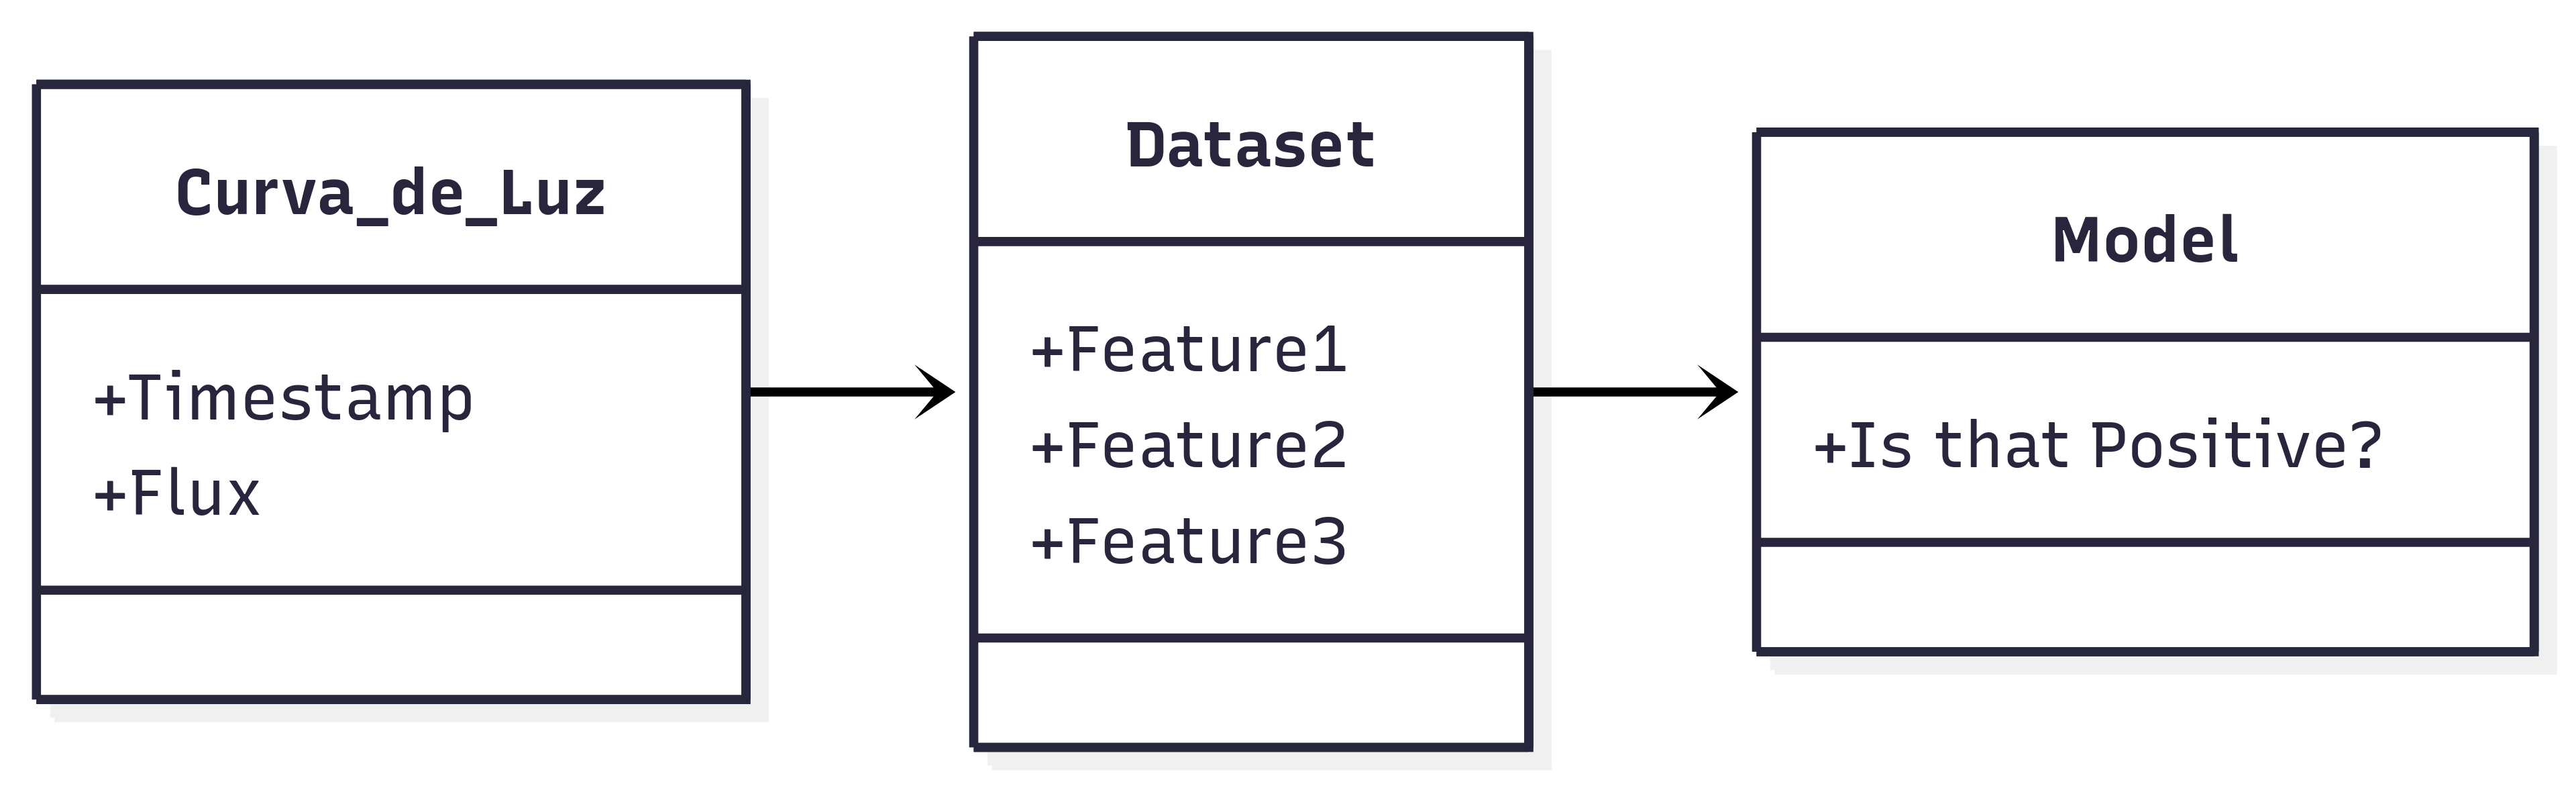
\includegraphics[scale=0.08]{pngs/diagrama_1.png}
\caption{Esquema da \textit{pipeline}: as curvas de luz são convertidas em vetores de características; o treinamento utiliza essas características, e não as séries temporais brutas.}
\label{fig:diagrama_pipeline}
\end{center}
\end{figure}

% -----------------------------------------------------------------------------
\section{Aquisição e armazenamento dos dados}
\label{sec:aquisição}

\subsection{Fontes de dados}

As curvas de luz utilizadas neste trabalho provêm de duas origens principais.

\textbf{Grupo do Rio:} parte do conjunto foi obtida a partir do banco de dados em nuvem do Grupo do Rio, referente a campanhas de ocultações já analisadas na literatura: ocultação por Umbriel (satélite de Urano), observada em 2020 e analisada por \cite{Umbriel2020}, e ocultação por Chiron, observada em 2023 e analisada por \cite{Chiron2023}. Esses dados já possuem classificação (positiva ou negativa) e metadados consistentes. 

\textbf{VizieR:} a maior parte das curvas foi adquirida no portal VizieR (\textit{cdsarc.cds.unistra.fr}), catálogo \texttt{B/occ/asteroid}, totalizando centenas de curvas em formato \texttt{.dat}, contendo séries temporais de tempo e fluxo. Para cada entrada do catálogo, os pontos da curva são baixados via serviço \texttt{vizgraph} e armazenados localmente. Convém esclarecer uma possível confusão de escalas: os milhares de registros mencionados na Introdução referem-se às \textbf{imagens (quadros)} que cada observação produz, das quais se extrai \emph{uma} curva de luz por fotometria. O conjunto de dados deste trabalho é contado em \textbf{curvas}, não em quadros --- são centenas de curvas, que, somadas aos negativos artificiais e sintéticos, totalizam as 1693 amostras detalhadas na Seção~\ref{sec:config_experimental} (Capítulo~5).

O processamento e a integração dos dados foram realizados com as bibliotecas \texttt{Astropy} e \texttt{Astroquery} (leitura e consulta a catálogos astronômicos), \texttt{asyncio} e \texttt{aiohttp} (coleta assíncrona, reduzindo o tempo total de aquisição), e \texttt{Pandas} (manipulação tabular). Scripts em Python foram desenvolvidos para automatizar a busca, o download e a organização dos arquivos.

\begin{figure}[htbp]
\begin{center}
	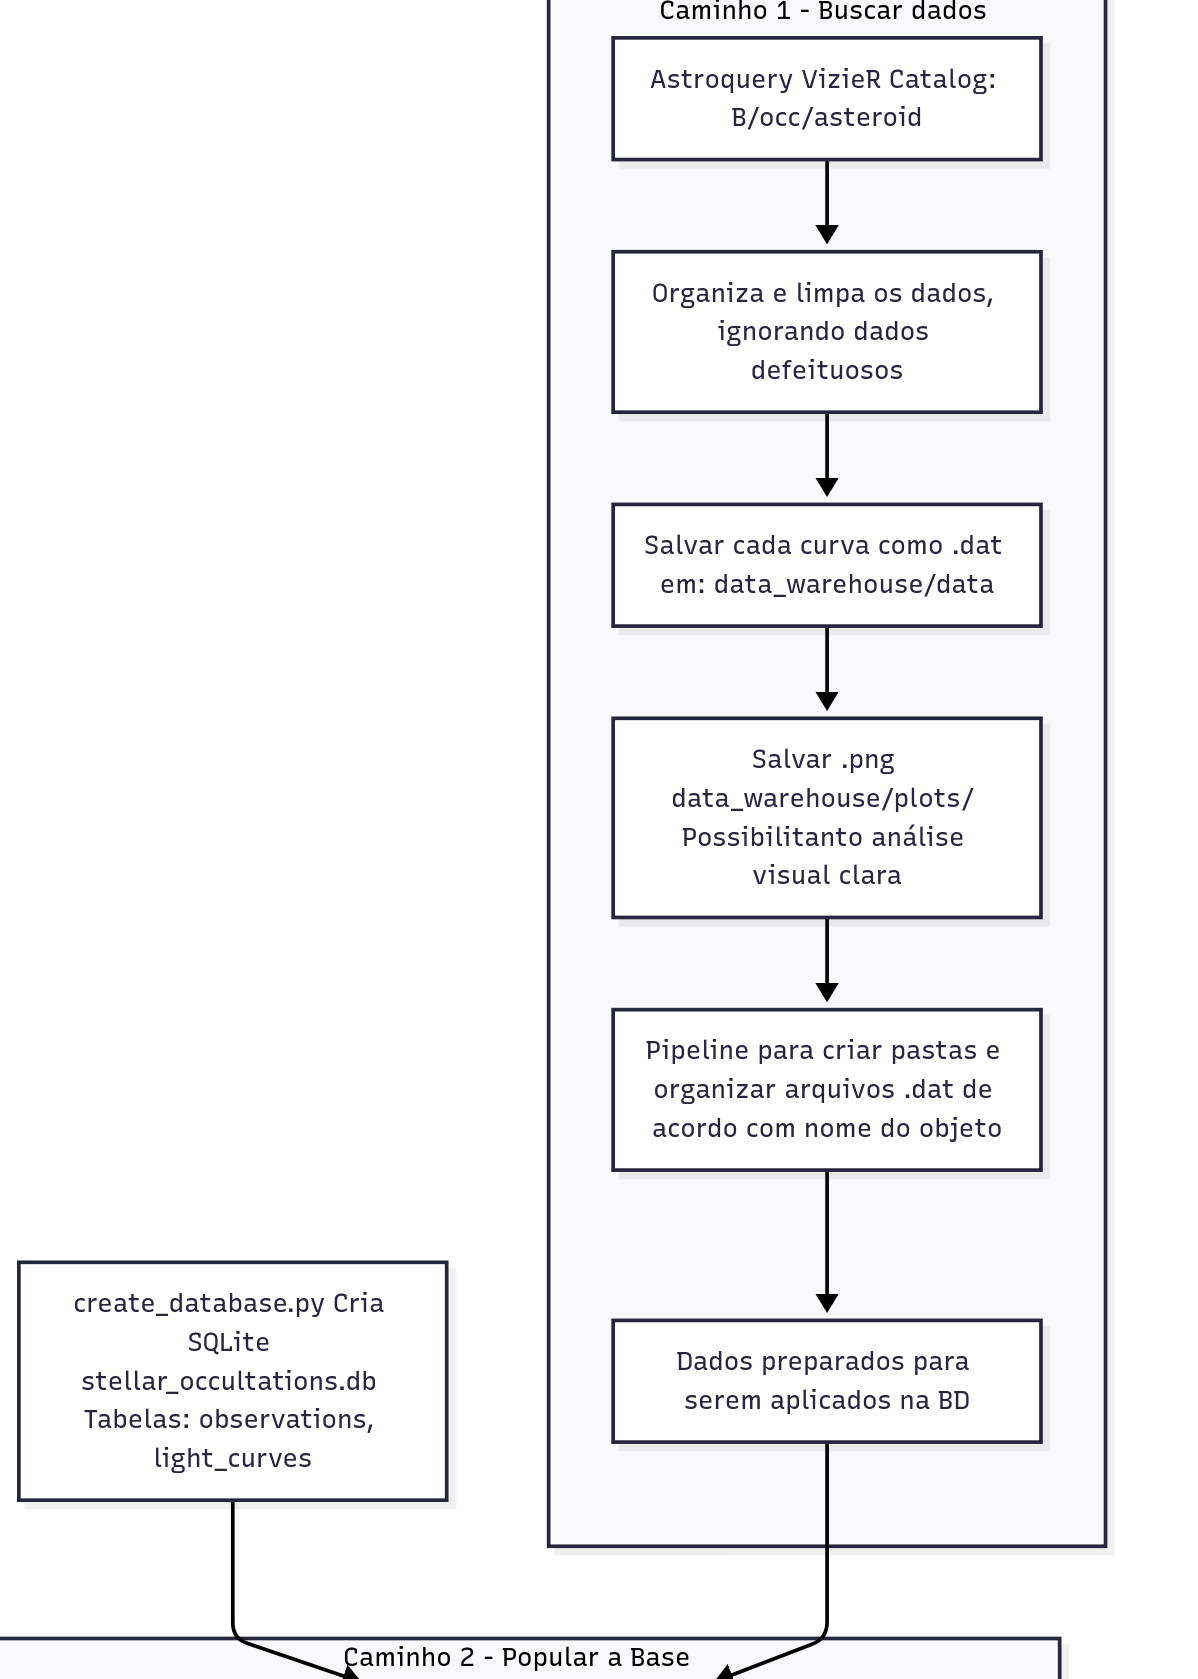
\includegraphics[scale=0.3]{pngs/fluxo1.png}
\caption{Fluxograma da aquisição e organização dos dados externos e da integração na etapa de inserção no banco de dados.}
\label{fig:fluxo1}
\end{center}
\end{figure}

\subsection{Estrutura do banco de dados}

O banco de dados relacional foi implementado em SQLite (\texttt{.db}) e estruturado em duas tabelas principais, garantindo integridade referencial e consultas eficientes.

\textbf{Tabela \texttt{observations}:} armazena informações gerais de cada observação: identificador único, nome do objeto ocultador, data da observação, portal de origem, nome do observador e metadados adicionais (incluindo a classificação do evento como ocultação positiva ou negativa, quando disponível).

\textbf{Tabela \texttt{light\_curves}:} contém os pontos individuais de cada curva de luz (tempo e fluxo), vinculados à observação correspondente por uma chave estrangeira (\texttt{observation\_id}). Assim, uma mesma observação pode possuir muitos pontos, mantendo a normalização do esquema.

Durante a inserção, buscou-se preservar ao máximo os valores originais, realizando apenas ajustes mínimos de consistência: uniformização de unidades quando necessário, checagem do alinhamento temporal e validação de metadados, sem alterar as características intrínsecas das curvas. A Figura~\ref{fig:fluxo2} resume o fluxo de consolidação do banco.

\begin{figure}[htbp]
\begin{center}
	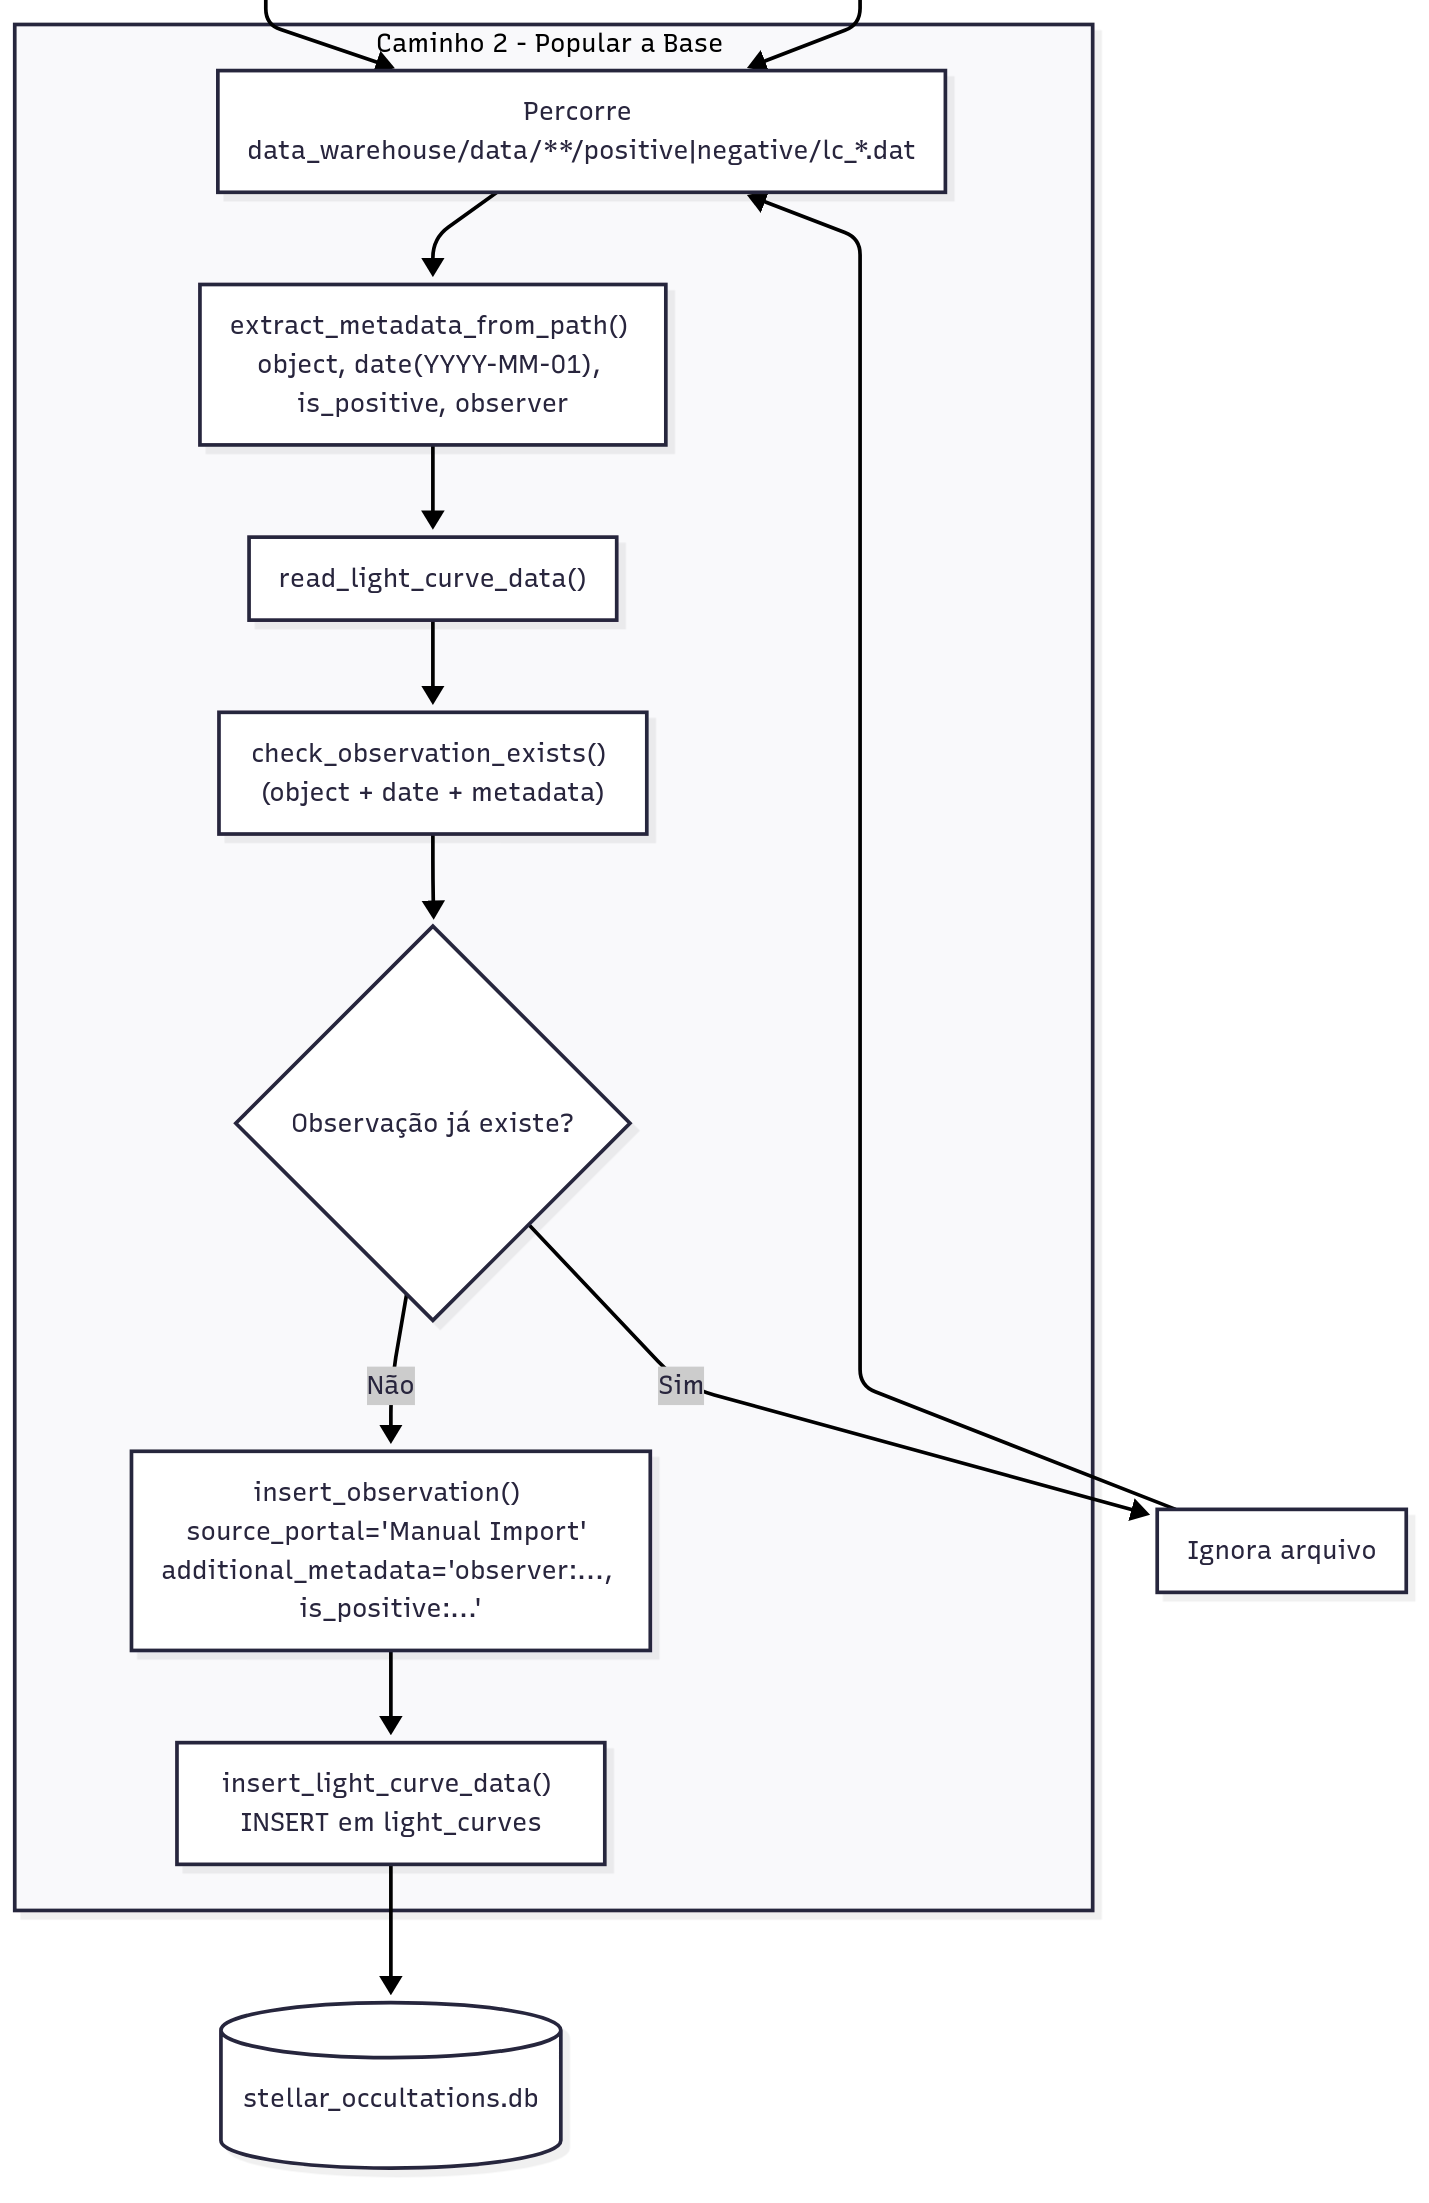
\includegraphics[scale=0.3]{pngs/fluxo2.png}
\caption{Fluxograma da \textit{pipeline} responsável pela consolidação do banco de dados.}
\label{fig:fluxo2}
\end{center}
\end{figure}

% -----------------------------------------------------------------------------
\section{Acesso aos dados e normalização}
\label{sec:acesso}

Após a consolidação no banco, um módulo dedicado (\textit{data access}) é responsável por consultar as curvas, filtrá-las por critérios (objeto, data, tipo positivo/negativo) e prepará-las para as etapas seguintes.

\subsection{Consulta e classificação}

As curvas são identificadas como \textbf{positivas} (com evento de ocultação) ou \textbf{negativas} (sem evento) com base em metadados armazenados na tabela \texttt{observations} (campo de metadados adicionais). Essa classificação pode provir de análises prévias (como no caso do Grupo do Rio) ou de anotações inseridas durante a organização dos dados. No Grupo do Rio, os rótulos decorrem das análises publicadas nas campanhas citadas (Umbriel, Chiron), realizadas por especialistas do grupo; no VizieR, a classificação positiva/negativa provém dos curadores do catálogo \texttt{B/occ/asteroid}. Não há estudo formal de concordância entre anotadores neste trabalho; as métricas de desempenho reportadas no Capítulo 5 são, portanto, relativas a esse \textit{ground truth} e devem ser lidas com a ressalva de que erros ou inconsistências de rotulagem nos catálogos podem afetar tanto o treinamento quanto a avaliação dos modelos. Durante a organização dos dados não foram identificados casos confirmados de rótulo invertido (positiva rotulada como negativa ou vice-versa); contudo, como não se realizou uma reanálise independente de cada curva, não é possível descartar a existência de inconsistências pontuais herdadas dos catálogos de origem. O módulo de acesso permite listar objetos disponíveis, datas de observação por objeto e, para cada par objeto--data, recuperar as curvas com seus rótulos.

\subsection{Normalização do fluxo}

O fluxo fotométrico bruto varia em escala entre observações (diferentes telescópios, condições de céu, etc.). Para colocar todas as curvas em uma base comparável, aplica-se uma normalização que estima um \textit{baseline} (nível de fluxo fora da ocultação) e divide-se a série pelo valor desse baseline.

A estratégia adotada é a seguinte: a série temporal do fluxo é dividida em quatro segmentos contíguos (quartis em ordem temporal). Calcula-se a média de cada segmento; os dois segmentos com maior média são considerados representativos do nível fora da ocultação. O \textit{baseline} é definido como a média dessas duas médias. O fluxo inteiro é então dividido por esse baseline, de modo que, em curvas sem ocultação ou nos trechos externos à ocultação, o valor normalizado fique próximo de 1. Em curvas com ocultação, a região de queda aparece com valores inferiores a 1. Em casos degenerados (poucos pontos ou baseline inválido), recorre-se à média global do fluxo como alternativa. A normalização coloca todas as curvas em uma escala comparável, facilitando a convergência dos algoritmos e a interpretação de resíduos; em modelos de regressão, a análise de resíduos é um diagnóstico fundamental para verificar a aderência do modelo aos dados \citep{Morettin2010}. Esse procedimento é análogo a uma normalização ``pós-fotometria'', em que o nível de continuum já foi tratado.

\subsection{Remoção de \textit{outliers}}

Quando necessário, pontos extremos do fluxo podem ser removidos com base em um critério de z-score: para um limiar \(z_{\mathrm{lim}}\) (por exemplo, 3), pontos cujo fluxo se afasta da média da série por mais de \(z_{\mathrm{lim}}\) desvios padrão são descartados. Isso reduz o impacto de picos ou quedas espúrias pontuais (defeitos de leitura, raios cósmicos, etc.) sem alterar a estrutura geral da curva.

% -----------------------------------------------------------------------------
\section{Construção do conjunto de dados para aprendizado de máquina}
\label{sec:construção_dataset}

O \textbf{conjunto de dados} (dataset) é a tabela de exemplos (curvas de luz convertidas em vetores de características) com suas classificação verdadeira (positiva ou negativa), usada para treinar e avaliar os classificadores. Devido à escassez de curvas negativas nos catálogos disponíveis, adotaram-se duas estratégias complementares: recorte de segmentos sem ocultação a partir de curvas positivas e geração de curvas sintéticas negativas com o simulador físico de Gomes-Ferrante \& Braga-Ribas~\citep{Simulator}. Os detalhes de cada estratégia são descritos nas subseções seguintes.

\subsection{Tamanho e composição do conjunto de dados}

Para interpretar sobreajuste, significância das métricas e generalização no Capítulo 5, é essencial conhecer o tamanho e a composição do conjunto utilizado. A composição final (quantidade de curvas positivas, negativas do banco, negativos artificiais por recorte manual, curvas sintéticas, total de amostras e proporção treino/teste) é apresentada na Seção 5.2 (Configuração experimental), onde os números dos experimentos são detalhados junto com a distribuição por fonte.

\subsection{Curvas positivas e negativas do banco}

As curvas classificadas como positivas são obtidas do banco via consultas que filtram observações com rótulo correspondente. As curvas negativas são obtidas da mesma forma. O número de curvas negativas ``nativas'' (observações realmente sem ocultação) costuma ser menor que o de positivas em muitos catálogos; daí a necessidade de estratégias complementares para ampliar a classe negativa.

\subsection{Recorte de segmentos negativos a partir de curvas positivas}

Uma forma de obter exemplos negativos de alta qualidade é recortar, das próprias curvas positivas, os trechos \textbf{fora} da região de ocultação (antes da imersão e depois da emersão). Esses segmentos representam o mesmo tipo de sinal (mesmo telescópio, mesma estrela, mesma noite) sem o evento, e portanto são bons candidatos a negativos.

O procedimento adotado foi o seguinte: para cada curva positiva, identifica-se a região de ocultação (por exemplo, pontos com fluxo normalizado abaixo de um limiar, e.g.\ 0,78). Os segmentos antes e depois dessa região são candidatos a negativos. Cada segmento é apresentado ao operador para revisão manual: aceitar (incorporar como negativo artificial) ou rejeitar. Quando um ou mais segmentos de uma curva positiva são aceitos, a curva positiva original é excluída do conjunto de positivos usados no treino, para evitar que a mesma observação apareça tanto como positiva quanto como negativa (vazamento de informação). Essa abordagem, embora mais trabalhosa que um recorte totalmente automático, reduz o risco de viés e garante que os negativos artificiais correspondam de fato a trechos sem ocultação.

\subsection{Curvas sintéticas negativas}

Para diversificar ainda mais a classe negativa e cobrir condições variadas de ruído e amostragem, foram incorporadas \textbf{curvas de luz sintéticas} geradas por um simulador físico. O simulador combina: (i)~geometria do evento (tempo, posição ao longo da corda); (ii)~difração de Fresnel nas bordas de imersão e emersão; (iii)~modelo de ruído (Poisson, ruído de leitura, cintilação atmosférica); (iv)~normalização pós-fotometria. Para a classe negativa, são geradas curvas sem evento (ou com diâmetro efetivo nulo), submetidas ao mesmo tipo de ruído e normalização das curvas reais. As curvas sintéticas são exportadas em formato \texttt{.dat} e carregadas pelo módulo de construção do dataset, sendo tratadas como negativas. Essa etapa permite aumentar o tamanho e a variedade do conjunto de treino e melhorar a generalização do modelo em condições diversas \citep{Simulator}.

O conjunto final reúne, portanto: positivas do banco (excluindo as usadas para recorte), negativas do banco, negativos artificiais (segmentos recortados e aprovados) e curvas sintéticas negativas. Cabe destacar que o catálogo \texttt{B/occ/asteroid} do VizieR, principal fonte das curvas positivas, é um agregador público de campanhas independentes envolvendo diferentes corpos, observadores, telescópios, datas e localizações geográficas; a diversidade observacional do conjunto positivo é, portanto, intrínseca à natureza do catálogo, e não há fonte observacional única que possa enviesar essa classe. Os pontos onde existe acoplamento entre amostras são explicitamente assumidos e mitigados: (i)~os negativos artificiais herdam telescópio, estrela e noite da curva positiva da qual foram recortados, motivo pelo qual a positiva original é excluída do conjunto de treino; (ii)~as curvas sintéticas, geradas por simulador físico, podem apresentar características de ruído distintas das observações reais, limitação retomada e quantificada no Experimento~3 (Capítulo~5). Todas as curvas passam pela mesma etapa de extração de características, descrita na próxima seção.

% -----------------------------------------------------------------------------
\section{Engenharia de características}
\label{sec:features}

As curvas de luz são séries temporais (tempo \(\times\) fluxo). Os modelos de classificação utilizados neste trabalho (Regressão Logística, Random Forest, XGBoost, CatBoost) recebem \textbf{vetores numéricos}, não as séries brutas. Por isso, cada curva é convertida em um vetor de \textbf{características} (features) extraídas da série --- por exemplo, amplitude, mínimo do fluxo suavizado, distância entre centróides do K-means, etc. O resultado é uma tabela em que cada linha é uma curva e cada coluna é uma dessas grandezas. As características foram padronizadas (média zero, desvio unitário) \textbf{apenas para a Regressão Logística}, via \texttt{StandardScaler} --- o transformador da biblioteca \texttt{scikit-learn} \citep{ScikitLearn2011} que, para cada variável, subtrai a média e divide pelo desvio padrão do conjunto de treino ---, uma vez que a regularização $\ell_2$ é sensível à escala das variáveis \citep{geron2019maos}. Os modelos baseados em árvores (Random Forest, XGBoost, CatBoost) recebem as \textit{features} em escala original, pois são insensíveis a transformações monotônicas de cada variável.

\subsection{Estatísticas básicas do fluxo}

Seja \(F(t)\) a série de fluxo (preferencialmente normalizado) com \(N\) pontos. Definem-se:

\begin{equation}
\mu = \frac{1}{N} \sum_{i=1}^{N} F(t_i), \qquad
\sigma = \sqrt{\frac{1}{N - 1} \sum_{i=1}^{N} \left( F(t_i) - \mu \right)^2},
\end{equation}

\begin{equation}
F_{\min} = \min_{1 \leq i \leq N} F(t_i), \qquad
F_{\max} = \max_{1 \leq i \leq N} F(t_i).
\end{equation}

A amplitude da curva é \(\mathrm{Amp} = F_{\max} - F_{\min}\). Em curvas com ocultação, a amplitude tende a ser maior (queda pronunciada); em curvas apenas ruidosas, \(\sigma\) e a amplitude podem ser menores. O desvio padrão \(\sigma\) e a amplitude são portanto candidatos naturais a \textit{features} discriminativas.

\subsection{Suavização e médias móveis}

Para reduzir o ruído de alta frequência sem perder a forma geral da curva, aplica-se uma janela de suavização. A suavização atua como um filtro passa-baixa: atenua as flutuações rápidas ponto a ponto (componentes de alta frequência, associadas ao ruído) e preserva as variações lentas (baixa frequência), que descrevem a forma da ocultação. A janela é adaptativa ao tamanho da série: utiliza-se \(N/40\) para séries longas (ex.: \(N > 120\) pontos) e \(N/3\) para séries mais curtas, com mínimo de 3 pontos e ímpar para filtros simétricos. Com essa janela, calculam-se:

\begin{itemize}
	\item Média móvel do fluxo; extraem-se o máximo e o mínimo da série suavizada.
	\item Filtro de Savitzky-Golay (polinômio de ordem 2), que preserva melhor os picos e vales; do fluxo suavizado por Savitzky-Golay extraem-se máximo, mínimo e desvio padrão.
\end{itemize}

Essas medidas resumem o comportamento ``suave'' da curva e são menos sensíveis a flutuações pontuais.

\subsection{Max drawdown}

O \textit{max drawdown} é a maior queda do fluxo em relação ao máximo acumulado até cada instante:

\begin{equation}
\mathrm{drawdown}(i) = F(t_i) - \max_{1 \leq j \leq i} F(t_j), \qquad
\mathrm{Max\_Drawdown} = \min_i \, \mathrm{drawdown}(i).
\end{equation}

Em curvas com ocultação, o max drawdown tende a ser mais negativo; em curvas sem evento, permanece próximo de zero (apenas flutuações).

\subsection{K-means no fluxo suavizado}

Conforme definido na Seção~\ref{sec:kmeans} (Capítulo~3), o K-means é um algoritmo de agrupamento não supervisionado; nesta etapa, ele é empregado não como classificador, mas como \textbf{extrator de característica}. Aplica-se o K-means com \(K=2\) aos valores do fluxo suavizado (Savitzky-Golay), tratando cada ponto como um vetor unidimensional. A escolha de \(K=2\) é motivada pela física do problema: espera-se que uma curva com ocultação apresente dois regimes de fluxo --- o nível fora do evento (\textit{baseline}) e o nível rebaixado durante a queda. A \textbf{distância entre os dois centróides} resultantes é então usada como \textit{feature}: curvas com ocultação bem definida tendem a apresentar distância maior; curvas apenas ruidosas, distância menor.

\subsection{Derivadas}

A partir do fluxo suavizado, calculam-se a primeira e a segunda derivada (numericamente, e.g.\ via \texttt{np.gradient}). Uma ocultação típica produz picos negativos na primeira derivada (queda) e inflexões na segunda. São extraídas estatísticas dessas derivadas: mínimo, máximo, média, desvio padrão, assimetria (\textit{skewness}) e curtose da primeira derivada; mínimo, máximo e desvio padrão da segunda derivada. Essas \textit{features} capturam a ``forma'' da transição e ajudam a distinguir quedas reais de quedas espúrias ou ruidosas.

\subsection{Comparação entre quartis (testes estatísticos)}

A série é dividida em quatro quartis temporais. Para cada par de quartis, aplicam-se um teste \(t\) de Welch (diferença de médias) e um teste de Kolmogorov-Smirnov (K-S), que compara as funções de distribuição acumulada das duas amostras e fornece um \(p\)-valor sob a hipótese de que as distribuições são iguais \citep{Wall2003, Morettin2010}. Em curvas com ocultação, pelo menos um quartil (o que contém a queda) tende a diferir dos demais; os \(p\)-valores dos testes tendem a ser pequenos. Define-se então a \textit{feature} como o menor \(p\)-valor entre todos os pares, em escala logarítmica: \(-\log_{10}(p_{\min} + \epsilon)\), para evitar \(\log(0)\). Valores altos indicam forte evidência de diferença entre segmentos, compatível com a presença de um evento.

\subsection{Métricas de profundidade, duração e ajuste de modelos}

Além das \textit{features} descritas até aqui, a \textit{pipeline} incorpora um conjunto de métricas inspiradas em critérios observacionais discutidos em fóruns entre astrônomos amadores para análise de curvas difíceis de ocultação. Não há documento oficial que defina essas grandezas como critério definitivo para classificar uma curva como positiva; no texto referimo-nos a elas simplesmente como \textbf{métricas de profundidade, duração e ajuste de modelos}, isto é, grandezas adotadas neste trabalho e inspiradas em critérios práticos de análise, sem alegar que constituam definições formais consagradas na literatura. A implementação concreta segue o módulo de engenharia de características do projeto (arquivo \texttt{occ\_features.py}), cujas fórmulas são resumidas abaixo.

\textbf{Baseline.} O nível de fluxo fora da ocultação é estimado pela mediana da série: \(\mathrm{baseline} = \mathrm{mediana}(F)\). Em implementações alternativas pode-se usar a média dos pontos com fluxo acima da mediana. A mediana é robusta a \textit{outliers} --- valores extremos isolados, como quedas ou picos pontuais causados por raios cósmicos ou defeitos de leitura ---, que pouco a deslocam, ao contrário do que ocorreria com a média.

\textbf{Profundidade do dip.} A queda do fluxo em relação ao baseline é
\begin{equation}
\mathrm{depth} = \max\big(0,\, \mathrm{baseline} - \min_i F(t_i)\big).
\end{equation}
Em curvas sem ocultação, \(\mathrm{depth} \approx 0\); em curvas com evento, \(\mathrm{depth}\) reflete a magnitude da queda.

\textbf{Desvio do baseline.} O desvio padrão \(\sigma_{\mathrm{baseline}}\) é calculado apenas sobre os pontos com fluxo \(\geq \mathrm{baseline}\) (fora do dip). Essa grandeza estima o \textbf{ruído fotométrico fora do evento}: a dispersão natural do fluxo medido quando não há ocultação, decorrente das incertezas de medição (ruído de fótons, de leitura e de cintilação atmosférica). Usá-la como referência evita contaminar a medida de ruído com a própria queda. Se houver poucos pontos acima do baseline, usa-se o desvio padrão de toda a série.

\textbf{SNR do dip.} Neste trabalho, define-se a razão sinal-ruído da queda como o quociente entre a profundidade do \textit{dip} e o ruído estimado fora do evento:
\begin{equation}
\mathrm{SNR\_dip} = \frac{\mathrm{depth}}{\sigma_{\mathrm{baseline}}}.
\end{equation}
Valores altos indicam queda significativa em relação ao ruído, compatível com evento real.

\textbf{Sequências abaixo do baseline.} Uma \textit{sequência} (\textit{run}) é um bloco consecutivo de índices em que \(F(t_i) < \mathrm{baseline}\). Ocultações típicas produzem uma sequência longa; ruído tende a sequências curtas ou isoladas. Define-se o \textbf{número de frames na maior sequência} como a quantidade de pontos do maior bloco consecutivo abaixo do baseline.

\textbf{Duração em segundos.} A duração da maior sequência é \(\Delta t = t_{\mathrm{fim}} - t_{\mathrm{início}}\), onde \(t_{\mathrm{início}}\) e \(t_{\mathrm{fim}}\) são os instantes do primeiro e do último ponto dessa sequência. Essa grandeza está ligada à geometria do evento (tamanho do objeto, velocidade).

\textbf{Fluxo mínimo e razão.} Sejam \(F_{\min} = \min_i F(t_i)\) e a razão \(F_{\min}/\mathrm{baseline}\) (quando \(\mathrm{baseline} > 0\)). Em curvas normalizadas com ocultação, a razão tende a ser menor que 1.

\textbf{Chi² do modelo constante.} O modelo ``sem evento'' assume fluxo constante igual ao baseline. Define-se
\begin{equation}
\chi^2_{\mathrm{const}} = \sum_i \frac{(F_i - \mu)^2}{\sigma^2},
\end{equation}
com \(\mu = \mathrm{baseline}\) e \(\sigma\) uma escala robusta dos resíduos (por exemplo, MAD --- mediana do valor absoluto dos desvios em relação à mediana).

\textbf{Chi² do modelo ``square well''.} O modelo com dip assume nível constante fora da janela da maior sequência e nível constante (média do fluxo) dentro da janela, em formato de ``poço retangular''. A predição \(\mathrm{pred}_i\) vale \(\mathrm{baseline}\) fora da janela e a média do fluxo na janela dentro dela. Define-se
\begin{equation}
\chi^2_{\mathrm{sw}} = \sum_i \frac{(F_i - \mathrm{pred}_i)^2}{\sigma^2}.
\end{equation}

\textbf{Razão chi².} A grandeza
\begin{equation}
\chi^2_{\mathrm{ratio}} = \frac{\chi^2_{\mathrm{const}}}{\chi^2_{\mathrm{sw}}}
\end{equation}
mede o ganho de ajuste ao incluir o dip: valores \(\chi^2_{\mathrm{ratio}} > 1\) indicam que o modelo com dip explica melhor os dados. Na implementação, a razão é limitada ao intervalo \([0{,}1,\, 10]\) para evitar valores extremos. Curvas sem dip tendem a \(\chi^2_{\mathrm{ratio}} \approx 1\).

No dataset gerado pela \textit{pipeline}, essas grandezas aparecem em colunas cujos nomes no código possuem o prefixo \texttt{Occ\_} (de \textit{occultation}), por exemplo \texttt{Occ\_depth}, \texttt{Occ\_duration\_s}. No texto, tratamos todas elas como métricas de profundidade, duração e ajuste de modelos.

\subsection{Resumo das \textit{features}}

O vetor final de \textit{features} inclui: amplitude e desvio padrão do fluxo; máximo e mínimo da média móvel e do Savitzky-Golay; max drawdown; distância entre centróides do K-means no fluxo; mínimos \(-\log_{10}(p)\) dos testes \(t\) e K-S entre quartis; as estatísticas das derivadas primeira e segunda listadas acima; e as métricas de profundidade, duração e ajuste de modelos (profundidade do dip, SNR do dip, duração em segundos da maior sequência abaixo do baseline, número de frames na maior sequência, desvio padrão do baseline, fluxo mínimo, razão fluxo mínimo/baseline, \(\chi^2\) do modelo constante, \(\chi^2\) do modelo square well, razão \(\chi^2_{\mathrm{const}}/\chi^2_{\mathrm{sw}}\)). Todas as colunas de \textit{features} são numéricas; metadados como identificador da curva e rótulo (positivo/negativo) são mantidos em colunas separadas e não são usados como entrada do classificador. O resultado da etapa de engenharia de características é um arquivo tabular (por exemplo, \texttt{dataset\_final.csv}) em que cada linha é uma curva e as colunas são as \textit{features} mais o rótulo e o identificador.

% -----------------------------------------------------------------------------
\section{Treinamento e avaliação dos modelos}
\label{sec:treinamento}

\subsection{Preparação dos dados e divisão treino/teste}

O dataset final é carregado a partir do arquivo gerado na etapa anterior. As colunas de metadados (identificador da curva, fonte, rótulo) são separadas das colunas de \textit{features}. Valores faltantes (NaN) são preenchidos pela \textbf{mediana} calculada no conjunto de treino (\texttt{SimpleImputer} com \texttt{strategy='median'}), estratégia robusta a \textit{outliers}. O rótulo binário (ocultação presente = 1, ausente = 0) é definido como variável alvo.

A divisão entre treino e teste pode ser feita de duas formas:

\begin{enumerate}
	\item \textbf{Divisão estratificada:} os dados são divididos aleatoriamente em conjunto de treino e conjunto de teste (por exemplo, 80\% treino e 20\% teste), mantendo a proporção das classes em cada parte (\textit{stratified split}). Uma semente fixa (\textit{random state}) é utilizada na divisão para garantir reprodutibilidade; a mesma semente (ou sementes documentadas) é empregada no treinamento de cada modelo (Regressão Logística, Random Forest, XGBoost, CatBoost), de modo que os experimentos sejam reproduzíveis.
	\item \textbf{Seleção manual de teste:} um subconjunto de curvas é fixado como conjunto de teste (por exemplo, curvas de um objeto ou data específicos). O restante compõe o treino. Essa opção é útil para avaliar a generalização para cenários de interesse conhecido.
\end{enumerate}

As métricas de desempenho (acurácia, precisão, sensibilidade, F1-score, AUC-ROC) são calculadas no conjunto de teste e reportadas no Capítulo 5. Quando a escolha de hiperparâmetros for feita por validação cruzada, pode-se reportar também a média e o desvio padrão da métrica nas dobras de validação, para dar noção da variabilidade; no conjunto de teste, as métricas são reportadas como valor único, condicionado à divisão treino/teste adotada.

\subsection{Modelos utilizados}

Foram utilizados quatro algoritmos de classificação supervisionada, descritos no Capítulo 3:

\begin{itemize}
	\item \textbf{Regressão Logística:} classificador linear probabilístico com regularização \(\ell_2\) (Ridge) ou \(\ell_1\) (Lasso); hiperparâmetro de força de regularização (\(C\) ou \(\alpha\)) escolhido via validação cruzada.
	\item \textbf{Random Forest:} ensemble de árvores de decisão com \textit{bagging}; hiperparâmetros típicos incluem número de árvores (\textit{n\_estimators}), profundidade máxima (\textit{max\_depth}) e peso das classes (\textit{class\_weight='balanced'}) para lidar com desbalanceamento.
	\item \textbf{XGBoost:} \textit{gradient boosting} com árvores; controle de profundidade, taxa de aprendizado (\textit{learning\_rate}), subamostragem de linhas e colunas.
	\item \textbf{CatBoost:} outro algoritmo de \textit{boosting}, com opção de ponderação automática das classes (\textit{auto\_class\_weights='Balanced'}).
\end{itemize}

Os valores concretos dos hiperparâmetros utilizados nos experimentos (e eventual busca em grade ou validação cruzada) estão documentados no Apêndice~\ref{ap:hiperparametros}. A escolha desses modelos deve-se ao seu bom desempenho em problemas de classificação com dados tabulares, à interpretabilidade (importância de variáveis) e à disponibilidade em bibliotecas estáveis (scikit-learn, XGBoost, CatBoost). Para quantificar a interpretabilidade, a \textbf{importância das variáveis} é calculada da seguinte forma: nos ensembles baseados em árvores (Random Forest, XGBoost, CatBoost), utiliza-se a importância por \textbf{queda média na impureza} (Gini) em cada divisão em que a variável participa, conforme fornecido pelas respectivas bibliotecas; na Regressão Logística, utilizam-se os coeficientes estimados (em valor absoluto). Os rankings e as magnitudes das importâncias são apresentados e discutidos no Capítulo 5.

\subsection{Métricas de avaliação}

As definições formais das métricas de classificação binária utilizadas neste trabalho --- acurácia, precisão, sensibilidade, F1-score, $F_\beta$-score, AUC-ROC e curva precision-recall --- foram apresentadas na Seção~\ref{sec:metricas_avaliacao} (Capítulo~3). Aqui, discutem-se as escolhas específicas adotadas na \textit{pipeline} à luz do problema de detecção de ocultações.

Em problemas de detecção de eventos, a matriz de confusão e as métricas dela derivadas permitem avaliar a capacidade do modelo de tomar decisões confiáveis \citep{Cazeneuve2023}. A \textbf{curva ROC} visualiza o \textit{trade-off} entre a taxa de verdadeiros positivos (sensibilidade) e a taxa de falsos positivos à medida que o limiar de decisão varia; a \textbf{área sob a curva} (AUC-ROC) resume a capacidade de ordenação do modelo de forma independente do limiar escolhido \citep{AUC-curve}. Em problemas com \textbf{classe positiva rara} --- isto é, quando os exemplos de interesse (positivos) são minoria expressiva frente aos negativos ---, a \textbf{curva precision-recall} pode ser mais informativa, pois não é inflada pelo grande número de verdadeiros negativos.

No contexto desta dissertação, em que os dados são desbalanceados (muitas curvas sem ocultação), a \textbf{acurácia} sozinha pode ser enganosa, conforme ilustrado pelo exemplo numérico do Capítulo~3. Para detecção de ocultações estelares, a \textbf{sensibilidade} tem prioridade, pois não perder eventos raros é essencial; a \textbf{precisão} evita excesso de falsos positivos que sobrecarregariam a triagem humana. O \textbf{F1-score} equilibra precisão e sensibilidade e é adequado para comparar os quatro modelos em cenário desbalanceado. A \textbf{AUC-ROC} avalia a capacidade de separação das classes de forma global.

\subsection{Fluxo de treinamento e persistência}

O fluxo de treinamento é: (1)~carregar o conjunto de dados; (2)~separar as colunas de características das colunas de rótulo (positivo/negativo); (3)~dividir em treino e teste (por exemplo, 80\% treino, 20\% teste); (4)~treinar cada um dos quatro modelos no conjunto de treino; (5)~avaliar cada modelo no conjunto de teste, calculando as métricas acima; (6)~gerar visualizações (curvas ROC, matrizes de confusão, importância de cada variável); (7)~salvar os modelos ajustados e um resumo das métricas em disco. Os modelos salvos podem ser carregados depois para classificar novas curvas ou para comparação com outras configurações. Os resultados numéricos e as figuras são a base da discussão do Capítulo 5.

% -----------------------------------------------------------------------------
%\section{Considerações finais do capítulo}
%\label{sec:consideracoes_cap4}

Este capítulo apresentou a metodologia completa da \textit{pipeline} de detecção de ocultações estelares em curvas de luz: desde a aquisição e o armazenamento em banco relacional até o treinamento e a avaliação de classificadores. A arquitetura em etapas (aquisição \(\to\) acesso e normalização \(\to\) construção do dataset \(\to\) engenharia de características \(\to\) treinamento) permite reproduzir o fluxo e estendê-lo com novas fontes de dados, novas \textit{features} ou novos modelos. A combinação de dados reais (VizieR, Grupo do Rio), negativos artificiais obtidos por recorte manual e curvas sintéticas visa um conjunto de treino equilibrado e representativo. A extração de características baseada em estatísticas, suavização, derivadas e testes entre quartis fornece uma representação vetorial adequada aos modelos de árvore e à Regressão Logística utilizados. No próximo capítulo, são apresentados os resultados obtidos com os quatro modelos treinados (Regressão Logística, Random Forest, XGBoost, CatBoost), incluindo comparação de desempenho, análise de importância das variáveis e discussão sobre generalização e possível overfitting.
